\documentclass[a4paper, 12pt]{article}
%%%%%%%%%%%%%%%%%%%%%%%%%%%%%%%%%%%%%%%%%%%%%%%%%%%%%%%%%%%%%%%%%%%%%%%%%%%%%%%%%%%%%%%%%%%%%%%%%%%%%%%%%%%%%%%%%%%%%%%%%%%%%%%%%%%%%%%%%%%%%%%%%%%%%%%%%%%%%%%%%%%%%%%%%%%%%%%%%%%%%%%%%%%%%%%%%%%%%%%%%%%%%%%%%%%%%%%%%%%%%%%%%%%%%%%%%%%%%%%%%%%%%%%%%%
% autocompile publish

\usepackage{math-hse}
\usepackage{tikz}
\title{Дополнительные задачи 1}
\renewcommand{\thesubsection}{\arabic{subsection}}

\date{16.01.2020}
\begin{document}

\noindent{\textit{Данный листок содержит задачи повышенной сложности, которые 
можно самостоятельно решать на семинаре, если разбираемые у доски 
задачи кажутся слишком простыми. Рекомендуется приступать к этим задачам 
только в том случае, если основной материал по теме усвоен и отработан. 
Задачи, аналогичным данным, не входят в формы контроля, 
предусмотренные на курсе. }}\\

\noindent{\textit{Решение этих задач засчитывается как 
выступление у доски в случае, если студент приводит верное 
или частично верное решение и готов устно рассказать его преподавателю. }}

\begin{problem}
План очень маленького города $N$ изображен на Рис.~1.  
В этом городе $3 \times 2$ прямоугольных квартала, которые разделены 
между собой прямыми улицами.

\begin{figure}[ht!]
\centering
\begin{tikzpicture}
\draw[help lines] (0,0) grid (3,2);
\node [left] at (0,0) {$A$};
\draw[fill, red] (0,0) circle [radius=0.06];
\node [right] at (3,2) {$B$};
\draw[fill, red] (3,2) circle [radius=0.06];
\end{tikzpicture}
\caption{город $N$}
\end{figure}

\begin{enumerate}
\item  Изобразите все
возможные пути из точки $A$ в точку $B$, считая, что странник хочет идти 
кратчайшим путем, то есть двигаться по сетке 
только слева направо или снизу вверх.  Сколько получилось путей?
\itemОтметьте на плане города все перекрестки, где странник 
должен делать выбор, куда ему пойти: направо или вверх (включая точку $A$ и 
исключая точку $B$). Сопоставьте каждому пути из предыдущего пункта 
последовательность из $0$ и $1$, где $0$ означает, что странник должен 
идти наверх, а $1$ -- что он должен идти направо.
Например, пути на Рис.~2 соответствует последовательность $10101$.
\end{enumerate}

\begin{figure}[ht!]
\centering
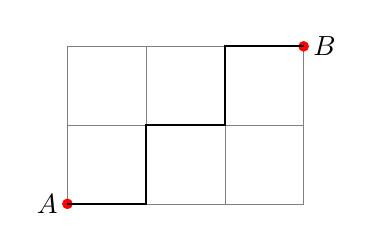
\begin{tikzpicture}
\draw[help lines] (0,0) grid (3,2);
\node [left] at (0,0) {$A$};
\draw[fill, red] (0,0) circle [radius=0.06];
\node [right] at (3,2) {$B$};
\draw[fill, red] (3,2) circle [radius=0.06];
\draw[thick] (0,0) -- (1,0) -- (1,1) -- (2,1) -- (2,2) -- (3,2);  
\end{tikzpicture}
\caption{пример пути из точки $A$ в точку $B$}
\end{figure}

\begin{statement}
Пусть есть прямоугольная сетка размера $n\times k$. Точка $A$ -- левый нижний угол сетки, 
а точка $B$ -- правый верхний угол этой сетки. Число путей из точки $A$ в 
точку $B$ при описанном выше способе движения по сетке
равно числу перестановок из $n$ единиц и $k$ нулей:
$$
P(k, n) = C^n_{n+k} = \frac{(n+k)!}{n!~k!}.
$$
\end{statement}

\noindent Проверьте, что число путей, найденных вами в первом пункте, совпадает 
с числом путей, посчитанным по предложенной формуле. Используя сведения, полученные выше, 
решите следующую задачу.\medskip\\

\noindentВсе дороги города $M$ проходят по сетке, состоящей
из прямоугольников размера $k \times l$, где $k$ и $l$ -- 
целые неотрицательные числа (Рис.~3).
Парк обозначен точкой $P(0, 0)$, 
кофейня -- точкой $C(m, n)$.

\begin{figure}[ht!]
\centering
\scalebox{0.72}{
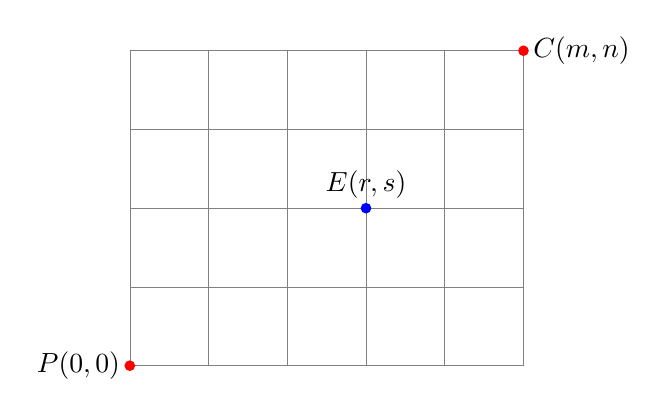
\begin{tikzpicture}
\draw[help lines] (0,0) grid (5,4);
\node [left] at (0,0) {$P(0, 0)$};
\draw[fill, red] (0,0) circle [radius=0.06];
\node [right] at (5,4) {$C(m,n)$};
\draw[fill, red] (5,4) circle [radius=0.06];
\node [above] at (3,2) {$E(r,s)$};
\draw[fill, blue] (3,2) circle [radius=0.06];
\end{tikzpicture}}
\caption{город $M$}
\end{figure}

\noindentГруппа друзей в день выборов кратчайшим путем 
направляется из парка в кофейню. 
В точке $E(r, s)$ находится избирательный участок. 

\begin{enumerate}
\item Найдите вероятность того, что друзья, не знающие об избирательном 
участке, смогут посетить его, если будут выбирать путь от парка до кофейни наугад.
\item При $m=6$, $n=4$, $r=3$ найдите значение $s$, определяющее наиболее выгодное 
расположение избирательного участка (с точки зрения посещения его жителями).
\end{enumerate}
\end{problem}

\begin{problem}
В круг радиуса $r$ вписан квадрат. 
Середины сторон этого квадрата соединены линиями, как показано на Рис.~4. 
В круг бросают четыре точки. Чему равна вероятность того, что ровно одна точка 
попадет в закрашенную область?
\end{problem}

\begin{figure}[ht!]
\centering
\scalebox{0.7}{
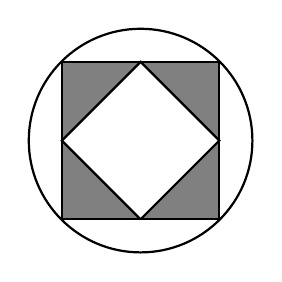
\begin{tikzpicture}
\draw[help lines] (0,0) grid (2,2);
\draw [thick] (1,1) circle [radius=1.42];
\draw [fill=gray,thick] (0,0) rectangle (2,2);
\draw [fill=white,thick] (1,0) -- (0,1) -- (1,2) -- (2,1) -- (1,0);
\end{tikzpicture}}
\caption{иллюстрация к задаче 2}
\end{figure}

\noindentЗадачи и пояснения базируются на следующих источниках: 

\begin{itemize}
\item Кочетков Е.С., Смерчинская С.О. Теория вероятностей в задачах и упражнениях. -- М.: Форум, 2008.
\item Виленкин Н. Я., Виленкин А.Н., Виленкин П.А. Комбинаторика. -- М.: МНЦМО, 2013.
\end{itemize}
\end{document}

